

\chapter{Discussion and Future Work}
\label{Discussion}

\section{Introduction}
\label{Discussion:Intro}

\section{Participatory approaches}
\label{Discussion:RQ1}
\begin{quote}
\textbf{    Research Question 1:
}    
\textit{    “How can we use participatory design approaches to provide meaningful and engaging experiences for people with dementia?”}
\end{quote}

Throughout the thesis, I addressed participatory design approaches in various ways. Chapter four examined a series of participatory design approaches to engage with people with dementia and their families. Through working closely with the families, I adapted traditional participatory methods to fit the needs of the participants, such as creating family days out in which participants would take part in walking interviews. Following on from this work, I was motivated to explore how to broaden these participatory methods to function within the context of larger-scale community events seen in chapter five - that prompted me to explore how hackathons could provide a creative and inclusive space for the public to engage the topic of dementia. 

However, while I gained reasonable interest from designers, developers and students, the event significantly under-represented people with dementia and their care partners. The failure to represent and involve people with dementia in public engagement had multiple knock-on effects on teams' outputs. Still, it provided an opportunity to reflect on the appropriateness of hackathon structures for people with dementia and propose alternatives for collaborative design events. Finally, in chapter seven, I worked with people with dementia, designers, and developers to understand how these different stakeholders may collaborate in building technology. With this in mind, two considerations that arise in responding to the research question are: a) designing for contested realities and b) how we design for research to practice.

\section{Ethical implications in Dementia and HCI}
\label{Discussion:RQ2}
\begin{quote}
\textbf{    Research Question 2:
}    
\textit{    “What are the ethical implications for people with dementia to participate in HCI research?”}
\end{quote}
Across all the studies in this thesis, there has been ongoing ethical implications in how we involve and perceive people with dementia in HCI research. In particular, chapters four and six delve into such challenges in several ways. For chapter four,  I describe initial insights into my understandings of representation within dementia that encompasses my time at Silverline Memories and reflections on family history of dementia. As I explained at the end of chapter four discussion, the critical area that I felt remained underexamined was the ethical implications apparent in our work as a community of practice. This led to chapter six, where I invited 22 HCI and dementia researchers to reflect on their everyday experiences of working with people with dementia and the complexities that may arise in technology or institutional ethics. Through this thesis, exploring these ethical challenges led to more profound insights into the ways we represent and acknowledge people with dementia, and exploration into the 'ruling relations' that shape people with dementia's experiences. 

\section{Supporting meaningful dialogue}
\label{Discussion:RQ3}
\begin{quote}
\textbf{    Research Question 3:
}    
\textit{    “How can we support meaningful dialogue between the public, designers, developers, and people with dementia?”}
\end{quote}
In my literature review on the representation of dementia in the public eye, it is common for people with dementia to be stigmatised surrounding their abilities to communicate and socialise with others. As discussed in chapter four, I adapted the interview approaches to suit the family's needs by co-design days out, which supported meaningful dialogue between myself and the families with dementia. However, on a more comprehensive approach to this research question, chapter five - DemVR, and chapter seven - designing a collaborative toolkit, directly considers ways to facilitate an engaging and meaningful dialogue between the public, designers, developers, and people with dementia. In both chapters, I facilitated conversations surrounding ways technology can promote dialogue between the public and people with dementia. Chapter five deployed an online platform - Ideaboard, where designers, developers, people with dementia and care partners could take part in short consultations to share ideas for VR experiences to be explored in the hackathon. As I report in the chapter, this was a disfavoured platform that was lacked the engagement I had hoped for. In the discussion, I highlight issues of participant disinterest and how the platform was not intentionally built with people with dementia in mind. 

For the final data chapter, I build upon these mistakes to consider what toolkits and technologies could we use to support dialogue between people with dementia and technologists. In conducting this work with designers, developers and people with dementia from the ground-up, the findings demonstrated two priorities for making meaningful dialogue between the different communities - acknowledgement in contribution and how individuals may want to engage with one another.

\section{Competing interests}
\label{Discussion:RQ4}
\begin{quote}
\textbf{    Research Question 4:
}    
\textit{    “What are the competing interests and expectations for dementia design research when involving multiple stakeholders - such as people with dementia, developers, designers and researchers?”}
\end{quote}
From the breadth of literature in HCI and dementia, there is a clear indication towards tailoring technology and design approaches to the needs and desires of people with dementia and their family [cite]. Additionally, throughout the entire thesis, I have explored the competing interests of several stakeholders who impact technology development, such as designers, developers and researchers. By broadening the public conversation around dementia and HCI, the thesis contributes a series of insights into ways we may support conversations between technologists and people with dementia; ways to design for designer and developer workflows; and the challenges in designing for when the reality of the person with dementia is contested. With this in mind, this final section regarding the research questions will discuss a) ways we might design for contested realities and b) constructing a 'we' community between multiple communities. 

\subsection{Designing for contested realities}
\label{RQ4:ContestedRealities}

\section{Future work}
\label{FutureWork}

\subsection{Future studies}
\label{FutureStudies}
The following section builds on the four data chapters to move beyond the abstract discussions found in the previous data chapters to present four exciting studies for future work within technology and dementia. Through these prospective studies, I have attempted to articulate what the abstract directions I have suggested may entail acting as inspiration for researchers who wish to build onto this work. In each future study, I propose a research question with a clear explanation of how this ties into prior work found in this thesis and why it is important for the future of dementia and HCI.

- this is not an exhaustive list, nor an attempt to design studies that will answer all the questions generated through this thesis. Rather, starting points for researchers who may be interested in exploring areas regarding VR, community design events, learning of ethics, and representation of dementia through storytelling. 

\subsubsection{Ageing in a virtual world}
\label{FutureStudyOne}
\begin{figure}[htp]
\centering
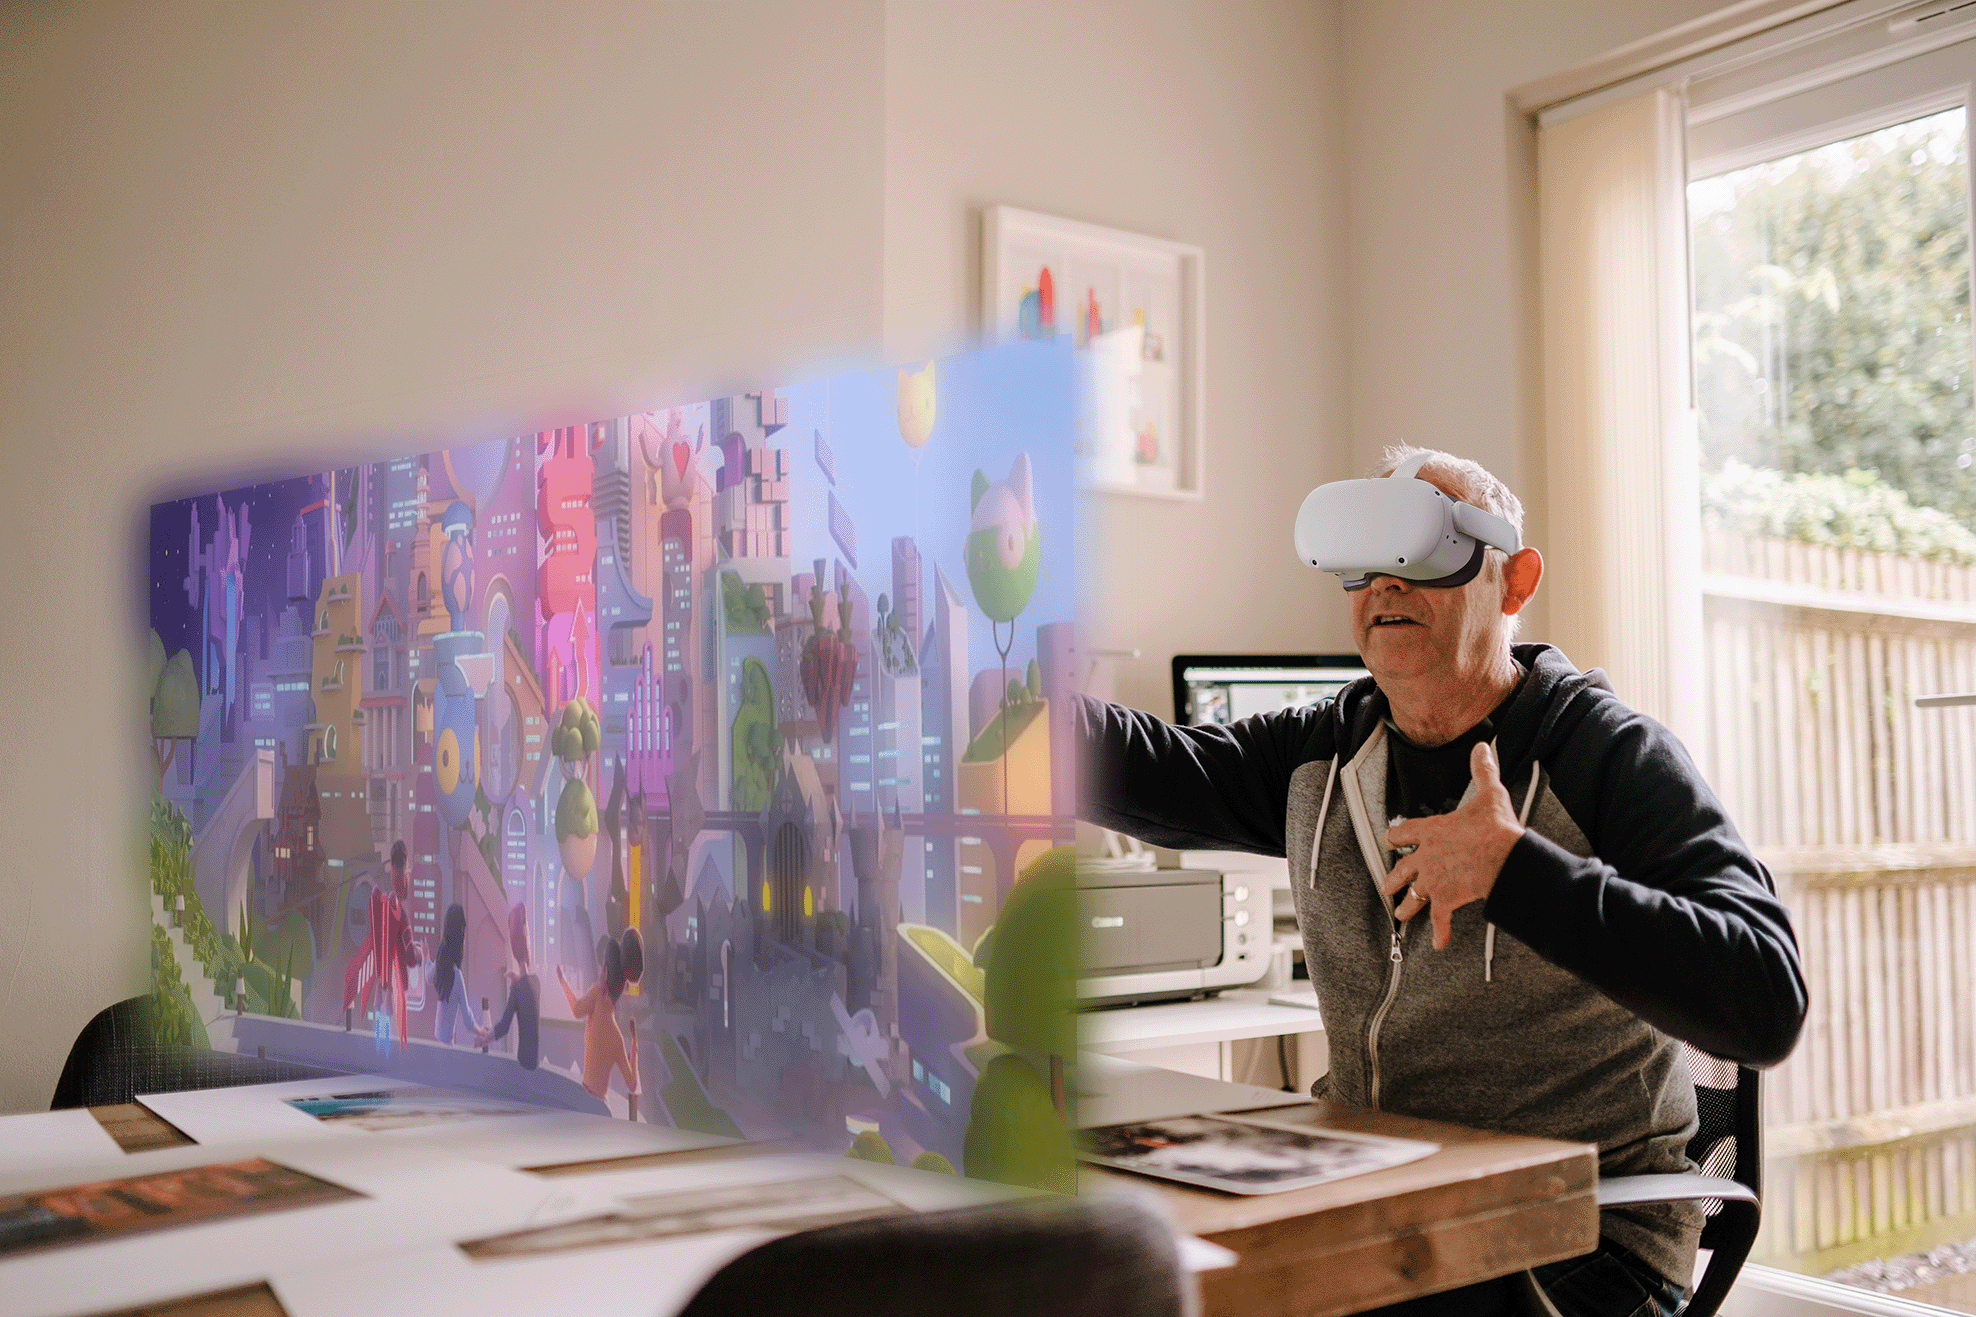
\includegraphics[width=1\linewidth]{Images/Discussion/Aging_in_VR.png}
\caption{Older adult exploring VR spaces}
\label{fig:Aging_VR}
\end{figure}
As mentioned in chapter four, the findings provided insight into several participants feeling a lack of confidence when getting out and about, due to the progression of their dementia. As we age, our body typically degrades as well, and people with dementia are often "reduced" to the bodily as their communicative abilities change and they move into care. Kontos describes much of the life of nursing homes in terms of their embodied potential. For instance, choosing to dress in specific ways, participating in the sleep-wake cycle of nursing homes, the attempts of care workers to transform (via various methods) residents into 'docile, dementing bodies'. However, Twigg et al. describe clothing provides a strong sense of selfhood and communication through embodied interactions: 
\begin{quote}
\textit{"Age has always been a one of the key structuring principles, and we should not be surprised to find it reflected at the bodily level in the clothes that people wear. Indeed, part of the wider role of clothes, as we noted, is to render social difference concrete and visible. But these traditional forms of age ordering are increasingly under pressure. The democratisation of fashion and the growth of involvement of older people in consumption are in the process of changing the nature of age ordering in dress in ways that point to wider shifts in the experience and understanding of later years." }[Clothing, identity and the embodiment of age]
\end{quote}

Twigg positions the body as a site for knowing the world - which can be fruitful when we consider designing VR experiences for people with dementia. With this in mind, a research question that has yet to be explored is \textbf{\textit{"How might we emphasise active ageing and representation of people with dementia through their designing of virtual avatars"}}. In chapter six - DemVR, multiple teams felt conflicted in fantasy elements and providing virtual hands and heads within the VR environment for different users. Ultimately, as described in the findings, the teams prioritised the safety of the person with dementia as they assumed people with dementia might feel uneasy with floating avatars that represent the user. However, in a recent study by Mendez [https://www.tandfonline.com/doi/full/10.3109/17483107.2014.889230], people with dementia communicated through their virtual avatars, including answering questions and conversing in the conversation between multiple virtual participants.

As VR continues to work with the popularity and investment into the 'metaverse', for some, using VR avatars is becoming an everyday interaction through virtual meeting rooms, playing online games with friends, to socialising in virtual spaces with strangers and friends. While there have been recent steps in improving virtual interactions between avatars, such as the new 'personal boundary' features to VR avatars to prevent others from creeping into the user's personal space, there is a lack of work into how we may age with these avatars. Do we preserve physical ailments and disabilities that often accompany dementia? Do we provide avatars that age over time in the same way our physical bodies do? Progressing in this area will mean careful co-design intervention that pays attention to the bodily as a means to communicate just as well as the verbal.

\subsubsection{Design with Inclusion}
\label{FutureStudyTwo}
\begin{figure}[htp]
\centering
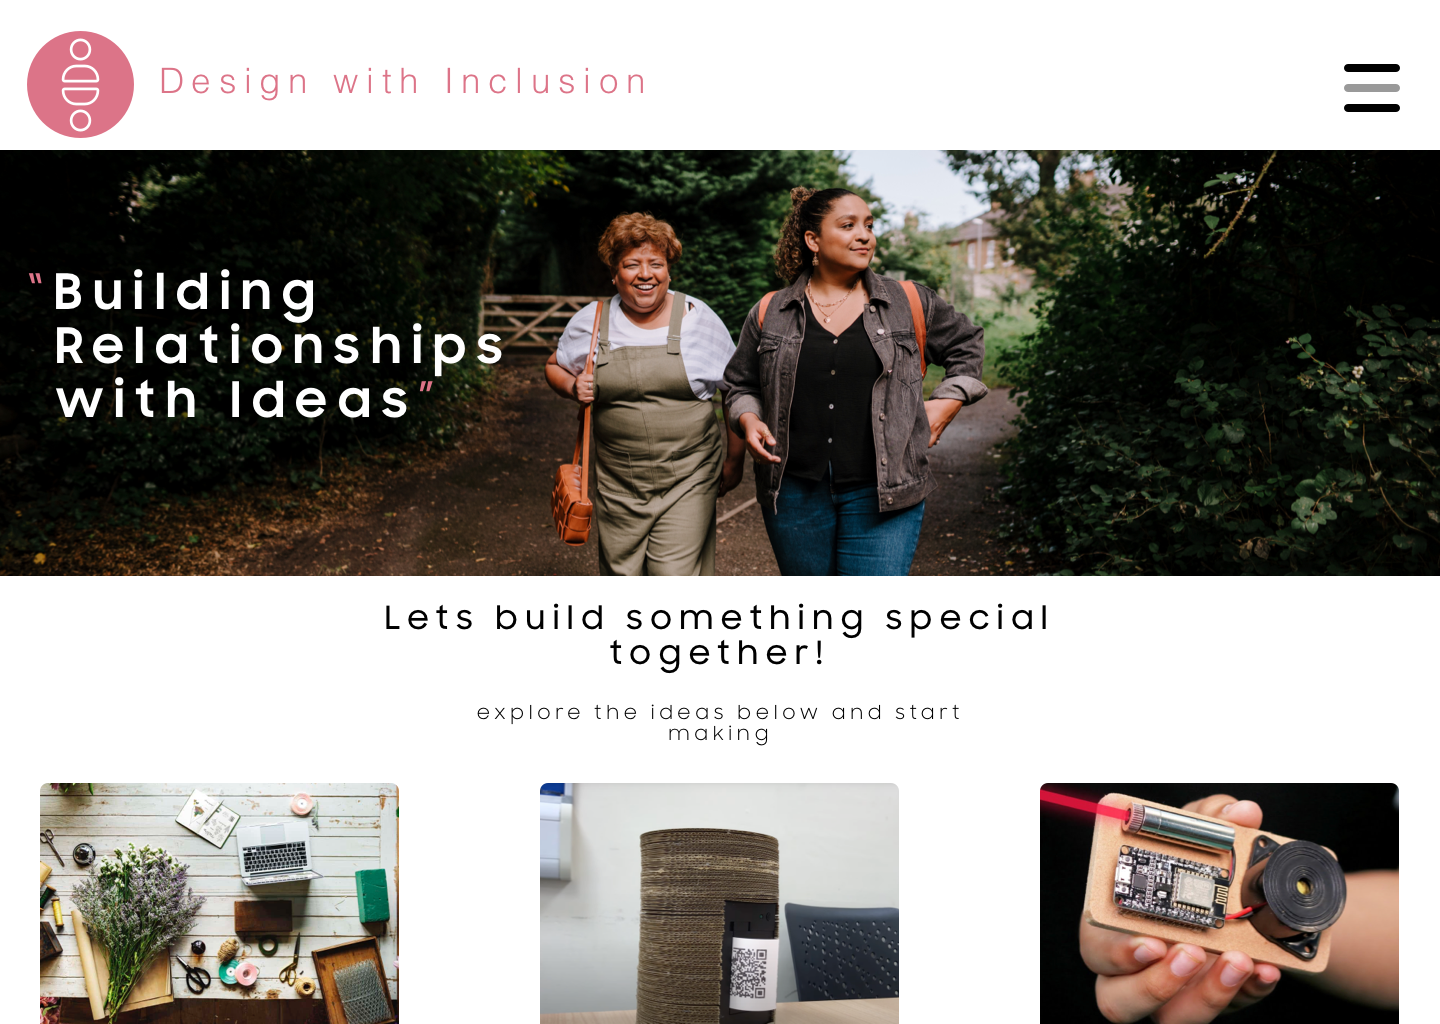
\includegraphics[width=1\linewidth]{Images/Discussion/Design_For_Inclusion.png}
\caption{Design with Inclusion website mockup}
\label{fig:DesignInclusion}
\end{figure}
One way forward in collaborative digital design for communities undergoing significant challenges might be to promote the growth of loosely coupled, companion 'communities of practice'. In chapter five - DEMVR, the makeup of many teams, which seemed to be themselves drawn from discrete, already existing communities; for example, undergraduates from the same computer science course; researchers from multimedia labs; and filmmakers. For design research for older age or in dementia, the idea of partnering communities together – for instance, partnering a cohort of design or technology students together with a community of older people, and having both mutually learn from one another – may hold promise. The UK-based 'FixEd' [36], for instance, has introduced a scalable learning programme called 'Fixperts' that targets schools and universities to engage their students in creative problem-solving that is rooted in the communities around them – for example, a student might engage with an older neighbour to innovate simple solutions that fit into their current lives, which help them get out of a car; or another student might work with someone experiencing a time-limited disability or injury to help them safely navigate their college campus. Capitalising on the ingenuity and availability of design, technology and engineering students looking for meaningful application areas, such programmes deliver small-scale, bespoke fixes for potentially large numbers of people. Similar ideas are seen at work in programmes such as TimeBanking [56], and even within studies previously cited such as Reuter et al's work [95], which made use of the resources a university is often rich in (e.g., technical competence, A/V equipment) to innovate within a radio programme for older people, leading them to encourage researchers 'to consider participatory action research as a method of assistance in itself, complimented by technical innovation to facilitate processes in this space'.

Given the interest in dementia as an area of interest for design and technology students, a study that might consider "How might we facilitate and promote different communities to 'partner-up' to share knowledge and skills?" In figure x, I have mocked up a website called 'Design with Inclusion' that builds up the challenges found in chapter five. It has been argued that older adults and people with dementia tend to adopt more DIY or ‘off the shelf’ products instead of using health and social care services. Although this largely stems from services not considering client’s needs, DIY solutions provide cheaper and tailored products that fulfil a particular problem [44]. Reflecting on the hackathon, an alternative approach would have been to let people with dementia and families to post ideas for DIY solutions that could have been built over a short period where designers and developers could share their skills in building the solution. Providing space for the different communities may have provided a more reciprocal relationship where designers learnt about dementia and lived experiences. In contrast, care partners and people with dementia would end up with a DIY project that they could use at home. Furthermore, by tailoring the interactions to be focused on personalised smaller scale products that tackle a particular challenge the user is facing, this may move away from fear for participants sacrificing their big hackathon idea to a university/organisation. By developing programmes of participation that are extended in time, organised around a common purpose, and provide meaningful benefits for student-practitioners, real, even incremental, change for a community of people with dementia. This may well be a more inclusive, ethical way to approach innovation and impact within this space.

\subsubsection{Suggestive guidance pack}
\label{FutureStudyThree}
\begin{figure}[htp]
\centering
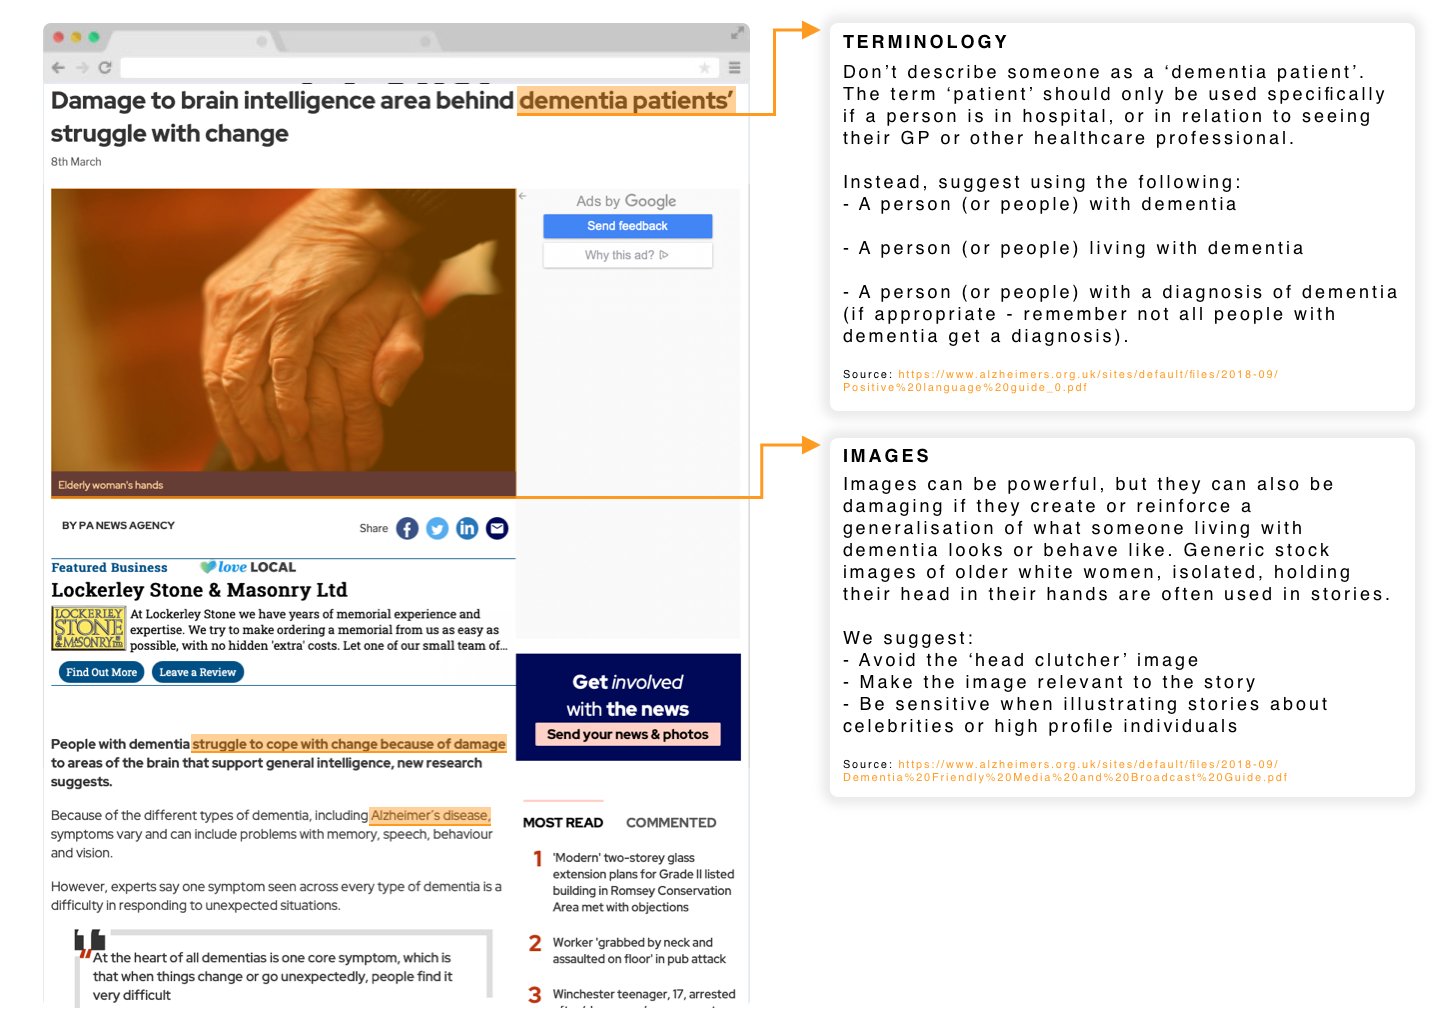
\includegraphics[width=1\linewidth]{Images/Discussion/Aware-AI.png}
\caption{Mockup of Suggestive guidance pack
 in action}
\label{fig:AwareAI}
\end{figure}
In the previous two chapters, I examined the ethical complexities that researchers, designers and developers face when designing with and for people with dementia. This work led to a series of unique insights into the ethical challenges of representing people with dementia and the co-creation of a lo-fi prototype toolkit for supporting communication and ethical decisions for designers, developers and people with dementia. One toolkit component that gained particular interest was 'suggestive guidance pack' found at reference. In this component, the tool would highlight negative labelling such as 'demented', or 'sufferer', and then suggest alternatives to improve the visual and textual representation of dementia (see how it may look like in fig.x). We could expand on this idea by "exploring how AI may assist in the teaching and representing people with dementia".

In recent years, AI-assisted tools have been widely used in the role of healthcare. These tools, have often been built to support the decision making of health records, insurance claims, and genome sequencing where the data is highly complex for human interpretation. Lysaght et al. describes a series of ethical challenges that arise in AI-assisted decision-making. They emphasise the importance of " the public would have even greater confidence that decisions made in the complex ICU setting were carefully considered by experts and supported advanced technology" [https://link.springer.com/article/10.1007/s41649-019-00096-0].

Lysaght raises important insights into AI decisions to have the necessary expertise back-up to provide confidence to whoever receives the information. Similarly, building upon the 'Suggestive Guidance Pack', people with dementia may be engaged with building the training data and guidance rules that the AI system build upon. For instance, people with dementia could vote and add recommendations for alternative suggestions for images that respectfully represent dementia.

In a similar vein to the early VR work found in chapter four, conducting work in AI and dementia may provide the opportunity to discover insights into how AI may support the social and political levels of dementia and HCI as opposed to the current stance of being used for pre-diagnostic and assessment studies. However, we must apply AI to social problems with an attentive and careful attitude, particularly when implementing the technology into sensitive settings that heavily rely on human contact and support. With this in mind, the future of AI design in dementia must require an interdisciplinary collaboration that is aware of the power relations amongst practitioners (that we have seen within this PhD)[https://dl.acm.org/doi/pdf/10.1145/3512346].

\subsubsection{Nothing about us, without us}
\label{FutureStudyFour}
\begin{figure}[htp]
\centering
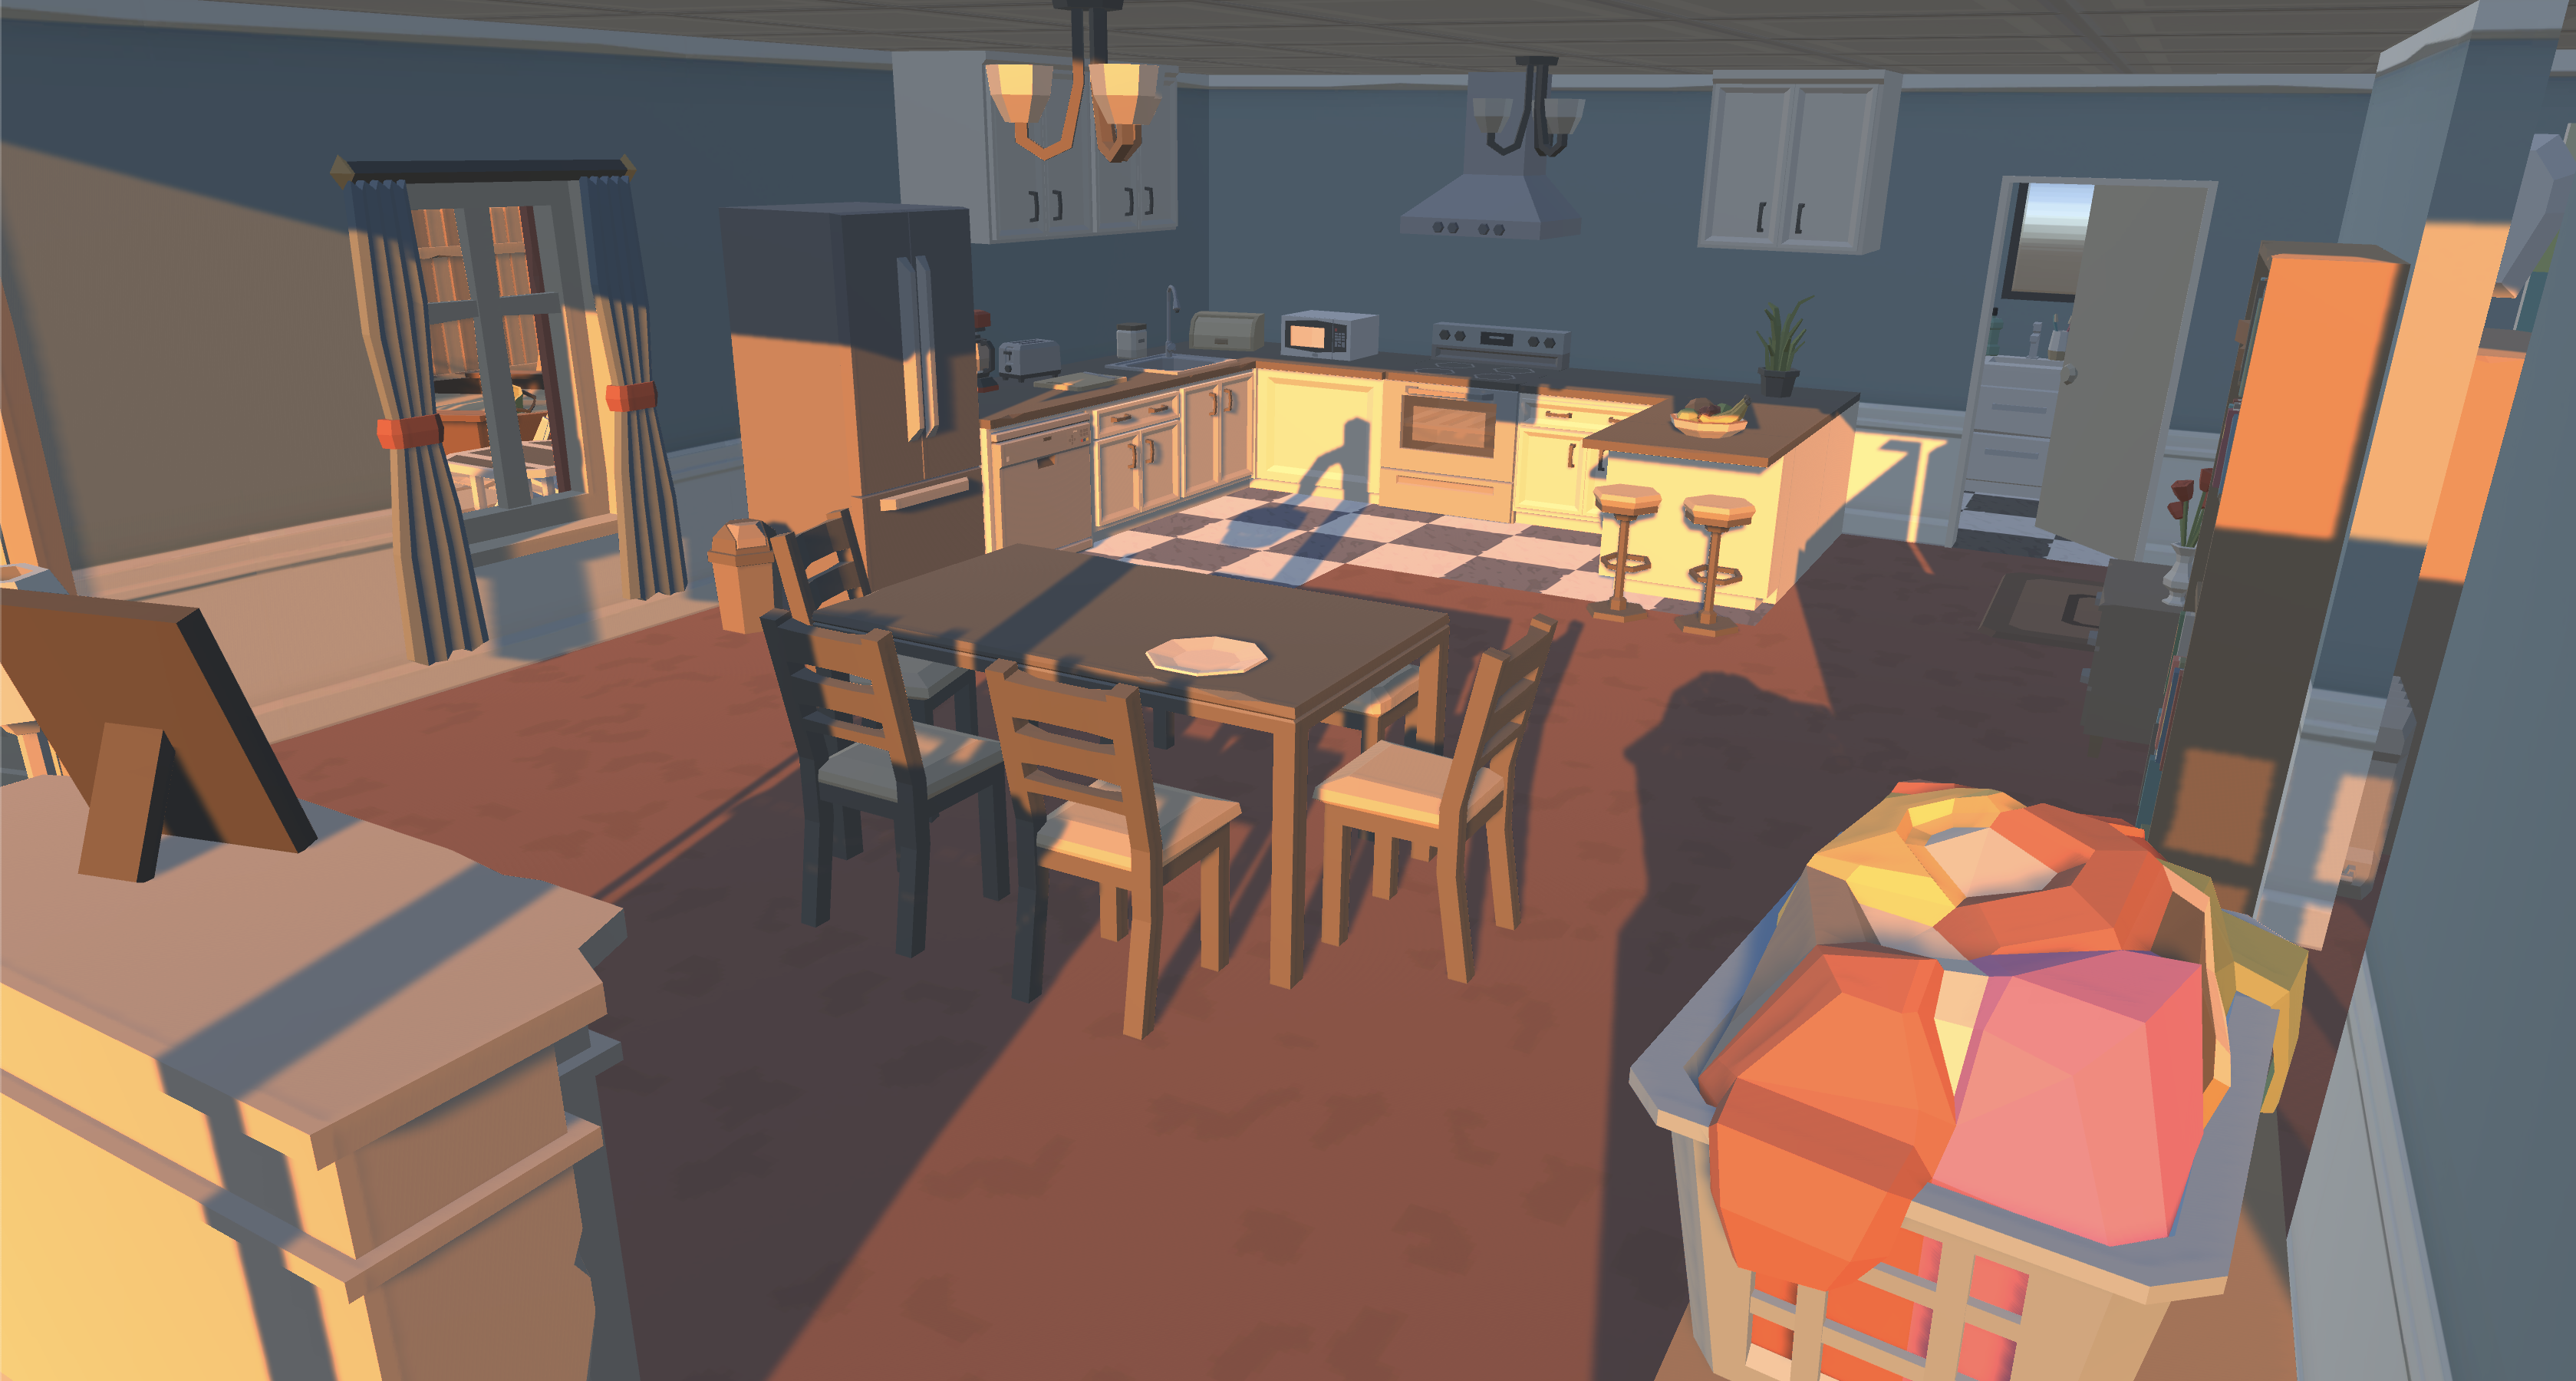
\includegraphics[width=1\linewidth]{Images/Discussion/Storytellling_Game.png}
\caption{Low-poly styling of a home for the game where the player can explore the person with dementia's story and learn about representation and stigma}
\label{fig:StorytellingLowPoly}
\end{figure}
In chapter seven's early stages of the toolkit, several workshops explored the idea of 'choose your own adventure' games to narrate the different experiences of dementia that will provide the public with immersive and meaningful explorations into what it means to live with dementia. Although this idea was not built upon in chapter seven, the use of games and other entertainment media formats may provide new ways to educate the public on the challenges and opportunities faced by experiences of dementia. 

Over the past decade, academia and best practice have presented a social and political perspective of what it means to live with dementia. However, while this may be a popular perspective, many academics or those within the dementia practice present within their work, this stance is radically different in the media portrayal. For instance, Bailey et al. explored how media coverage influences the public attitudes of dementia, describing media draws on "biomedical discourse conceals alternative discourses and ideologies, such as a discourse of political and social action which would reinforce dementia as a global issue". The authors highlight this is often due to the emphasis on finding a cure which undermines the importance of care and the social environment for people with dementia. Likewise, movies and games have often followed the similar pursuit of prioritising the focus on the biomedical stance, whether that is using dementia as a 'disease' that the characters tackle throughout the movie, or a VR game to convey the challenges of living with dementia in hopes to provide funding for a cure.

In order to tackle representation issues in the media, researchers may want to "explore how people with dementia may contribute to the design of media representation of dementia". One concept researchers may want to look into is how we may design interactive games that have been co-created by people with dementia to construct the type of experiences and narrative that games may provide (mock-up image in fig x.). From chapter 7, it was apparent that people with dementia want to be and are necessary to expressing a genuine representing of dementia but requires many different insights into the uniqueness of living with dementia. As popularised by several dementia advocates and the disability movement, the phrase 'nothing about us, without us' has become a popular saying and needs consideration in how media portrays dementia. This may be through a 'choose your own adventure game' to explore the different lives of people with dementia or act as a carer or friend to someone with dementia.While these types of media entertainment should focus on the discourse of living well with dementia to tackle the strong biomedical representation, I suggest we consider a more balanced view of the living with dementia that many of the participants I have worked with suggest. Additionally, although the living well with dementia perspective will develop a discourse that does not present a loss of agency, we must also acknowledge that they are challenges that come with dementia that requires necessary changes and alterations to the individuals', families', and friends' lives. 

\subsection{Final remarks}
\label{Discussion:FinalRemarks}